\documentclass[hyperref={pdfpagelabels=false},usepdftitle=false, xcolor = dvipsnames]{beamer}

\usepackage[T3]{fontenc}
\usepackage[utf8]{inputenc}
\usepackage[russian]{babel}

\usepackage{mhchem}
\usepackage{amssymb, amsmath}

\usepackage{tikz}
\usetikzlibrary{shapes.geometric, arrows, positioning, decorations.markings}
\usetikzlibrary{fit}
\usepackage{microtype}
\usepackage{framed}
\usetikzlibrary{decorations.pathmorphing,calc,backgrounds}

\usepackage{animate}

\usepackage{fixltx2e}
\usepackage{hyperref}

%\usetheme{Berkeley}
%\usetheme{Madrid} -- неплохо
%\usetheme{CambridgeUS}
%\usetheme{Singapore}
\usetheme{Warsaw}

\pdfmapfile{+sansmathaccent.map}

\title{Исследование бифуркаций в трехатомных гидридах методом классических траекторий}

\author{\small 
Финенко Артем \\[1ex] 
Научный руководитель: Петров С.В.}

\institute[MSU] % (optional, but mostly needed)
{
  МГУ им. М.В.Ломоносова \\
  Химический факультет
}

\date{23/12/2016}

\pgfdeclareimage[height=0.5cm]{university-logo}{../pictures/logo.jpg}
\logo{\pgfuseimage{university-logo}}

\newcommand\Fontvi{\fontsize{6}{7.2}\selectfont}

\beamertemplatenavigationsymbolsempty

\setbeamerfont{page number in head/foot}{size=\large}
\setbeamertemplate{footline}[frame number]
\setbeamertemplate{frametitle}[default][center]

% change font
\usefonttheme[onlymath]{serif}

% custom block environment
\newenvironment<>{varblock}[2][.9\textwidth]{%
  \setlength{\textwidth}{#1}
  \begin{actionenv}#3%
    \def\insertblocktitle{#2}%
    \par%
    \usebeamertemplate{block begin}}
  {\par%
    \usebeamertemplate{block end}%
  \end{actionenv}}

\tikzstyle{lagrange} = [rectangle, rounded corners, minimum width = 3cm, minimum height = 1cm, text centered, text width = 5cm, draw = black, fill=DarkOrchid!40]

\tikzstyle{equations} = [rectangle, rounded corners, text centered, draw = black, fill=green!30]

\tikzstyle{hamilton} = [rectangle, rounded corners, minimum width = 3cm, minimum height = 1cm, text centered, text width = 5 cm, draw = black, fill = Goldenrod!50]

\tikzstyle{result} = [rectangle, rounded corners, text centered, draw = black, fill = blue!30]

\tikzstyle{arrow} = [thick, ->, >=stealth]

\tikzstyle{vecArrow} = [thick, decoration={markings,mark=at position
   1 with {\arrow[semithick]{open triangle 60}}},
   double distance=1.4pt, shorten >= 5.5pt,
   preaction = {decorate},
   postaction = {draw,line width=1.4pt, white,shorten >= 4.5pt}]

\usepackage{caption}
\usepackage{subcaption}

\usepackage{dsfont} % uppercase
\usepackage{bbm} % lowercase

\newcommand{\bbA}{\mathds{A}}
\newcommand{\bbI}{\mathds{I}}
\newcommand{\bba}{\mathbbm{a}}

\begin{document}

\begin{frame}{\large
\begin{center}
Кафедра физической химии \\ Лаборатория строения и квантовой механики молекул
\end{center}}
  \titlepage
\end{frame}

\begin{frame}{Классический колебательно-вращательный гамильтониан I}
\begin{tikzpicture}[framed, font=\sffamily\small]
\node (lag1) [lagrange] {$\mathcal{L} = \mathcal{L}(\vec{r}_\text{1}^{\ \prime},  \cdots, \vec{r}_\text{n}^{\ \prime}, \dot{\vec{r}}_\text{1}^{\ \prime}, \cdots, \dot{\vec{r}}_\text{n}^{\ \prime})$};

\node (lag2) [lagrange, text width = 6 cm, below = 1 cm of lag1] {$\mathcal{L} = \mathcal{L} (\vec{r}_\text{1}, \cdots, \vec{r}_{\text{n-1}}, \dot{\vec{r}}_\text{1}, \cdots, \dot{\vec{r}}_{\text{n-1}})$};

\node (lag3) [lagrange, text width = 6 cm, below = 1 cm of lag2] {$\mathcal{L} = \mathcal{L}(\vec{R}_\text{1}, \cdots, \vec{R}_\text{n}, \dot{\vec{R}}_\text{1}, \cdots, \dot{\vec{R}}_{\text{n-1}}, \vec{\Omega})$};

\node (lag4) [lagrange, text width = 6 cm, below = 1 cm of lag3] {$\mathcal{L} = \mathcal{L}(\vec{q}_\text{1}, \cdots, \vec{q}_\text{s}, \dot{\vec{q}}_\text{1}, \cdots, \dot{\vec{q}}_\text{s}, \vec{\Omega})$};

\node (eq1) [equations, minimum width = 2cm, text width = 2cm, below right = 0.1 cm and 0.5 cm of lag1] {$\vec{r}_i^{\ \prime} = \vec{R} + \vec{r}_i$};

\node (eq2) [equations, minimum width = 2cm, text width = 2cm, below = 1.35cm of eq1] {$ \vec{r}_i = \mathbb{S} \vec{R}_i$};

\node (eq3) [equations, minimum width = 3cm, text width = 3cm, below right = 0.1 cm and -0.5 cm of lag3] {$\vec{R}_i = \vec{R}_i(q_\text{1}, \cdots, q_s)$};

\draw [vecArrow] (lag1) -- node (text1) [anchor = east, text width = 5cm] {\vspace*{-0.5cm} \begin{center}Переход в систему отсчета, связанную с центром масс \end{center}} (lag2);

\draw [vecArrow] (lag2) -- node (text2) [anchor = east, text width = 5cm] {\vspace*{-0.5cm} \begin{center}Переход в подвижную систему отсчета\end{center}} (lag3);

\draw [vecArrow] (lag3) -- node (text3) [anchor = east, text width = 5cm] {\vspace*{-0.5cm} \begin{center}Переход к обобщенным координатам\end{center}} (lag4);

\draw [arrow] (lag1) -| (eq1);
\draw [arrow] (eq1) |- ([yshift=4pt]lag2);
\draw [arrow] ([yshift=-4pt]lag2) -| (eq2);
\draw [arrow] (eq2) |- ([yshift=4pt]lag3);
\draw [arrow] ([yshift=-4pt]lag3) -| (eq3);
\draw [arrow] (eq3) |- (lag4);

\begin{scope}[on background layer]
  \node [fill = BurntOrange!20,fit= (lag1) (lag2) (lag3) (lag4) (text1) (text2) (text3) (eq1) (eq2) (eq3)] {};
\end{scope}
\end{tikzpicture}
\end{frame}

\begin{frame}{Классический колебательно-вращательный гамильтониан II}
\begin{center}
\begin{tikzpicture}[framed, font=\sffamily\small]
\node (lag1) [lagrange, text width = 6 cm, below = 1 cm of lag3] {$\mathcal{L} = \mathcal{L}(\vec{q}_\text{1}, \cdots, \vec{q}_\text{s}, \dot{\vec{q}}_\text{1}, \cdots, \dot{\vec{q}}_\text{s}, \vec{\Omega})$};

\node (ham1) [hamilton, below = 1.5 cm of lag1] {$\mathcal{H} = \mathcal{H}(\vec{q}_\text{1}, \cdots, \vec{q}_s, \vec{p}_\text{1}, \cdots, \vec{p}_s, \vec{J})$};

\node (eq1) [equations, below right = -0.2cm and 0.4cm of lag1] 
{$
\left\{
\begin{aligned}
\mathbf{J} &= \frac{\partial \mathcal{L}}{\partial \mathbf{\Omega}} \\
\mathbf{p} &= \frac{\partial \mathcal{L}}{\partial \dot{\mathbf{q}}}
\end{aligned}
\right.
$};

\draw [vecArrow] (lag1) -- node (text1) [anchor = east, text width = 3cm] {\vspace*{-0.5cm} \begin{center}Теорема Донкина \end{center}} (ham1);

\draw [arrow] (lag1) -| (eq1);
\draw [arrow] (eq1) |- (ham1);

\begin{scope}[on background layer]
  \node [fill = BurntOrange!20, fit = (lag1) (ham1) (eq1) (text1)] {};
\end{scope}
\end{tikzpicture}
\end{center}
\end{frame}

\begin{frame}{Модель трехатомного гидрида с деформационной степенью свободы}
  \begin{block}{}
	\begin{center}
	  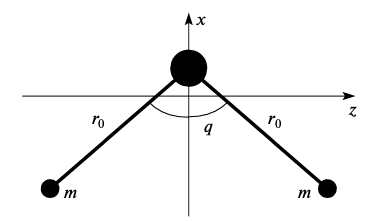
\includegraphics[width=0.6\textwidth]{../pictures/triatomic_fixed.png}
	\end{center}

	\vspace*{-1cm}
	\begin{gather}
	  \mathcal{H}(\vec{q}, \vec{p}, \vec{J}) = \frac{1}{2I_0} \left[ \frac{J_x^2}{1-\cos q} + \frac{J_z^2}{1 + \cos q} + \frac{J_y^2}{2} \right] + \frac{p^2}{I_0} + \notag \\
	  + \frac{1}{2I_0} \left( \frac{V_{-}}{1 - \cos q} + \frac{V_{+}}{1 + \cos q} \right), \quad I_0 = m r_0^2 \notag
	\end{gather}
  \end{block}
\end{frame}

\begin{frame}{Концепция поверхности вращательной энергии}
  \begin{varblock}[11cm]{}
	\begin{gather}
	  \left\{
	  \begin{aligned}
	    \left( \frac{\partial \mathcal{H}}{\partial \mathbf{q}} \right)_{\substack{\mathbf{q} = \mathbf{q}_e \\ \mathbf{p} = \mathbf{p}_e}} = 0 \\
		 \left( \frac{\partial \mathcal{H}}{\partial \mathbf{p}} \right)_{\substack{\mathbf{q} = \mathbf{q}_e \\ \mathbf{p} = \mathbf{p}_e}} = 0	     
	  \end{aligned}
	  \right.
	  \quad \implies \quad
	  \mathcal{H}_r \left( J_x, J_y, J_z \right) = \mathcal{H} \left( \mathbf{q}_e, \mathbf{p}_e, \mathbf{J} \right)
	  \notag \\
	  \mathcal{H}_r = \frac{1}{4I_0} \left[ \left( \sqrt{V_{+} + J_z^2} + \sqrt{V_{-} + J_x^2} \right)^2 + J_y^2 \right] \notag
	  \end{gather}
  \end{varblock}
  
\end{frame}

\begin{frame}{Поверхность вращательной энергии для модели с деформационной степенью свободы}
  \begin{varblock}[11cm]{}

	 \scriptsize \begin{gather}
	  E_r (\varphi, \theta; J) = \frac{1}{4I_0} \left[ \left( \sqrt{V_{+} + J^2 \cos^2 \theta} + \sqrt{V_{-} + J^2 \cos^2 \phi \sin^2 \theta} \right)^2 + J^2 \sin^2 \phi \sin^2 \theta \right] \notag \\
	  J_{cr.} = \sqrt{V_{-} - V_{+}} = I_0 \omega_0 \sqrt{ | \cos q_0 |} \notag
	  \end{gather}
	\vspace*{-0.5cm}
  	  \begin{figure}
  	    \begin{subfigure}{0.3\textwidth}
		  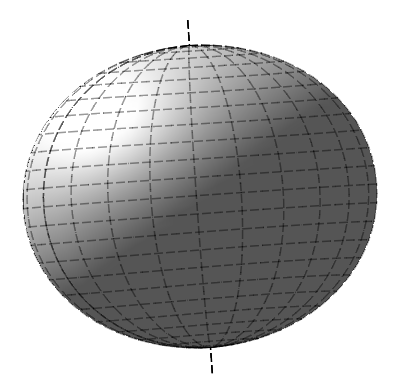
\includegraphics[width=\textwidth]{../pictures/Rigid_RES_10.png}
		  \caption{J = 10}
	    \end{subfigure}
	    \begin{subfigure}{0.3\textwidth}
		  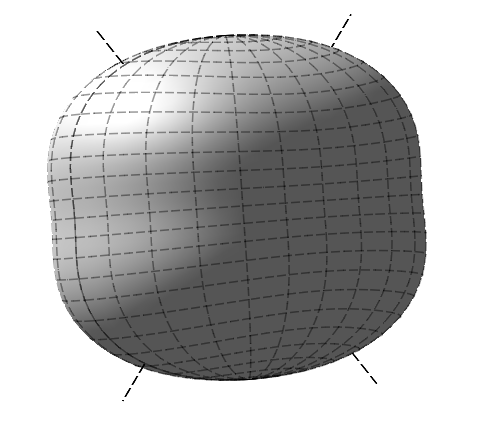
\includegraphics[width=\textwidth]{../pictures/Rigid_RES_30.png}
		  \caption{J=30}
		\end{subfigure}
		\begin{subfigure}{0.3\textwidth}
		  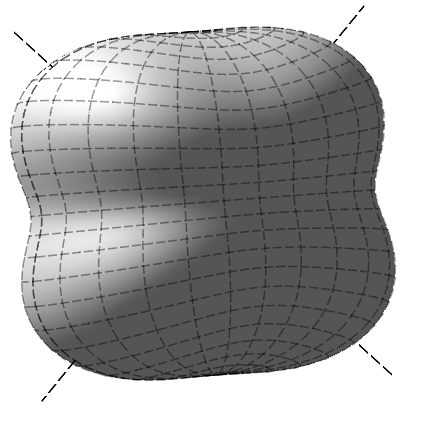
\includegraphics[width=\textwidth]{../pictures/Rigid_RES_50.png}
		  \caption{J=50}
		\end{subfigure}  
	  \end{figure}
  \end{varblock}    
\end{frame}

\begin{frame}{Полная система динамических уравнений}
\begin{center}
\begin{tikzpicture}
\node (eq1) [equations, minimum width = 4 cm, text width = 4 cm] 
{$
\left\{
\begin{aligned}
\dot{\mathbf{p}} &= \frac{\partial \mathcal{H}}{\partial \mathbf{q}} \\
\dot{\mathbf{q}} &= - \frac{\partial \mathcal{H}}{\partial \mathbf{p}} \\
\dot{\mathbf{J}} &+ \left[ \frac{\partial \mathcal{H}}{\partial \mathbf{J}} \times \mathbf{J} \right] = 0 
\end{aligned}
\right.
$};

\node (eq2) [equations, minimum height = 4cm, minimum width = 8cm, text width = 8cm, below right = 0.1cm and -3.5cm of eq1] 
{$
\left\{
\begin{aligned}
\dot{\mathbf{p}} &= \frac{\partial \mathcal{H}}{\partial \mathbf{q}} \\
\dot{\mathbf{q}} &= - \frac{\partial \mathcal{H}}{\partial \mathbf{p}} \\
\dot{\Phi} &= \left( \frac{\partial \mathcal{H}}{\partial J_x} \cos \Phi + \frac{\partial \mathcal{H}}{\partial J_y} \sin \Phi \right) \ctg \Theta - \frac{\partial \mathcal{H}}{\partial J_z} \\
\dot{\Theta} &= \frac{\partial \mathcal{H}}{\partial J_x} \sin \Phi - \frac{\partial \mathcal{H}}{\partial J_y} \cos \Phi
\end{aligned}
\right.
$};

\node (eq3) [equations, minimum height = 2 cm, minimum width = 3.5 cm, text width = 3.5 cm, right = 0.6 cm of eq1]
{$
\left\{
\begin{aligned}
J_x &= J \cos \Phi \sin \Theta \\
J_y &= J \sin \Phi \sin \Theta \\
J_z &= J \cos \Theta
\end{aligned}
\right.
$}; 

\draw [arrow] (eq1) -- (eq3);

\draw [arrow] 
([xshift=-8mm] eq3.south east) -- node [anchor = east, text width = 2cm] {\vspace*{-0.25cm}\begin{center} $J = \text{const}$ \end{center}} ([xshift=-11.9mm] eq2.north east);

\begin{scope}[on background layer]
  \node [fill = BurntOrange!20, fit = (eq1) (eq2) (eq3)] {};
\end{scope}
\end{tikzpicture}
\end{center}
\end{frame}

\begin{frame}{Система динамических уравнений для модельной системы}
  \begin{varblock}[11cm]{}
  \vspace*{-0.5cm}
	\scriptsize \begin{gather}
\left\{
\begin{aligned}
\dot{\Phi} &= \left( \frac{J \cos \Phi \sin \Theta}{I_0 ( 1 - \cos q)} \cos \Phi + \frac{J \sin \Phi \sin \Theta}{2I_0} \sin \Phi \right) \ctg \Theta - \frac{J \cos \Theta}{I_0 (1 + \cos q)} \\
\dot{\Theta} &= \frac{J \cos \Phi \sin \Theta}{I_0 (1 - \cos q)} \sin \Phi - \frac{J \sin \Phi \sin \Theta}{2I_0} \cos \Phi \\
\dot{q} &= 2	\frac{p}{I_0} \\
\dot{p} &= - \frac{\sin q}{2I_0} \left( \frac{J^2 \cos^2 \Theta}{(1 + \cos q)^2} - \frac{J \cos^2 \Phi \sin^2 \Theta}{(1 - \cos q)^2} \right) - \frac{1}{2I_0} \left( \frac{V_{+} \sin q}{(1 + \cos q)^2} - \frac{V_{-} \sin q}{(1 - \cos q)^2} \right)
\end{aligned}
\right. \notag
	\end{gather}
  \end{varblock}
\end{frame}

\begin{frame}{Траектории конца вектора углового момента в основном состоянии}
\begin{block}{}
\begin{figure}
  \begin{subfigure}{0.3\textwidth}
	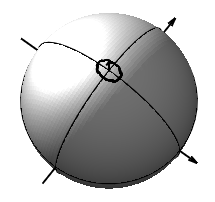
\includegraphics[width = \linewidth]{../pictures/rigid_base/plot_J=10n=0.png}
	\caption{J=10}
  \end{subfigure}
  \begin{subfigure}{0.3\textwidth}
    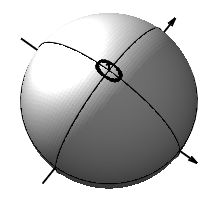
\includegraphics[width = \linewidth]{../pictures/rigid_base/plot_J=15n=0.png}
    \caption{J=15}
  \end{subfigure}
  \begin{subfigure}{0.3\textwidth}
    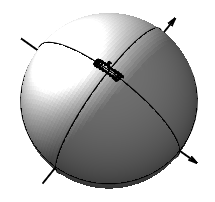
\includegraphics[width = \linewidth]{../pictures/rigid_base/plot_J=20n=0.png}
    \caption{J=20}
  \end{subfigure} \\
  \begin{subfigure}{0.3\textwidth}
     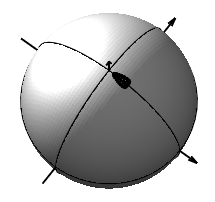
\includegraphics[width = \linewidth]{../pictures/rigid_base/plot_J=21n=0.png}
     \caption{J=21}
  \end{subfigure}
  \begin{subfigure}{0.3\textwidth}
    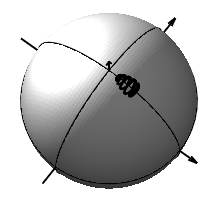
\includegraphics[width = \linewidth]{../pictures/rigid_base/plot_J=22n=0.png}
    \caption{J=22}
  \end{subfigure}
\end{figure}
\end{block}
\end{frame}

\begin{frame}{Полномерная модель трехатомного гидрида}
\begin{block}{Гамильтониан}
\scriptsize \begin{gather}
\mathcal{H} = \frac{1}{2} \left( \frac{J_x^2}{I_0 (1 - \cos q)} + \frac{J_y^2}{2 I_0} + \frac{J_z^2}{I_0 (1 + \cos q)} + 2 \frac{r_1^2 - r_2^2}{r_1^2 + r_2^2} \frac{J_x J_z}{I_0 \sin q} \right) + \frac{r_1^2 - r_2^2}{2m r_1^2 r_2^2} J_y p + \notag \\
+ \frac{p_1^2}{2m} + \frac{p_2^2}{2m} + \frac{p^2}{I_0} + U (r_1, r_2, q),
\quad I_0 = \frac{2m r_1^2 \cdot r_2^2}{r_1^2 + r_2^2} \notag
\end{gather}
\end{block}
\begin{block}{Потенциальная энергия}
\scriptsize \begin{gather}
\left[
\begin{aligned}
U(r_1, r_2, q) &= k (r_1 - r_0)^2 + k (r_2 - r_0)^2 + \frac{1}{2 I_1} \left( \frac{V_{-}}{1 - \cos q} + \frac{V_{+}}{1 + \cos q} \right) \\
U(r_1, r_2, q) &= D_e (1 - \exp (- a (r_1 - r_e))^2 + D_e (1 - \exp (- a (r_2 - r_e))^2 + \\
&+ \frac{1}{2 I_1} \left( \frac{V_{-}}{1 - \cos q} + \frac{V_{+}}{1 + \cos q} \right) ,
\end{aligned}
\right. \notag \\
I_1 = m r_0^2 \notag
\end{gather}
\end{block}
\end{frame}

\begin{frame}{\small Траектории конца вектора углового момента в полномерной модели с гармоническим потенциалом в основном состоянии}
  \begin{block}{}
	\begin{figure}
	  \begin{subfigure}{0.25\textwidth}
	    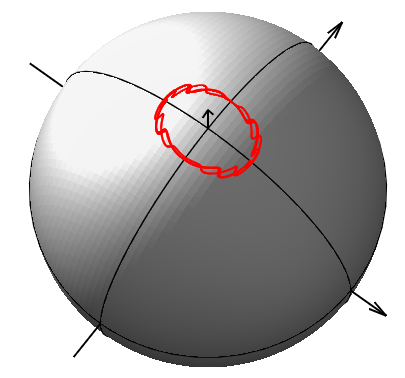
\includegraphics[width = \linewidth]{../pictures/HarmGroundState00/plot_J=10.png}
	    \caption{J=10}
	  \end{subfigure}
	  \begin{subfigure}{0.25\textwidth}
	    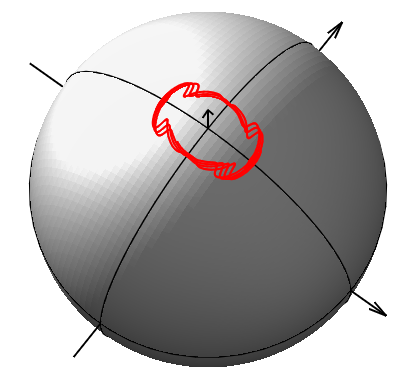
\includegraphics[width = \linewidth]{../pictures/HarmGroundState00/plot_J=15.png}
	    \caption{J=15}
	  \end{subfigure}
	  \begin{subfigure}{0.25\textwidth}
	    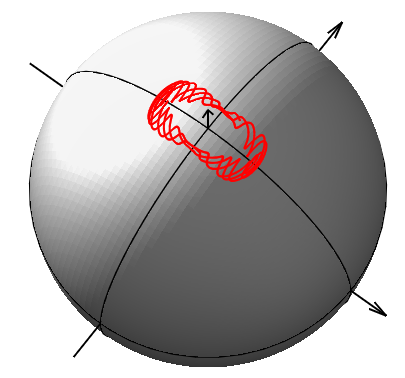
\includegraphics[width = \linewidth]{../pictures/HarmGroundState00/plot_J=20.png}
	    \caption{J=20}
	  \end{subfigure}
	  \begin{subfigure}{0.25\textwidth}
	    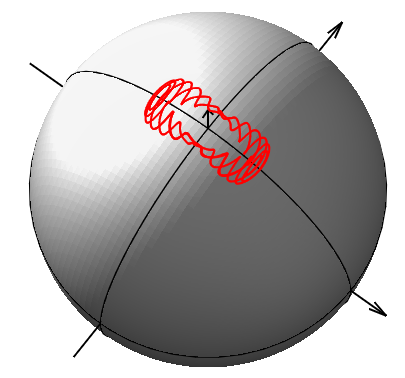
\includegraphics[width = \linewidth]{../pictures/HarmGroundState00/plot_J=22.png}
	    \caption{J=22}
	  \end{subfigure}
	  \begin{subfigure}{0.25\textwidth}
	    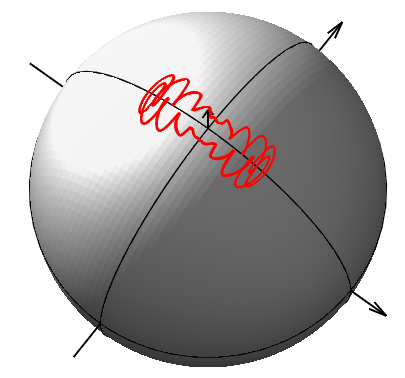
\includegraphics[width = \linewidth]{../pictures/HarmGroundState00/plot_J=24.png}
	    \caption{J=24}
	  \end{subfigure}
	  \begin{subfigure}{0.25\textwidth}
	    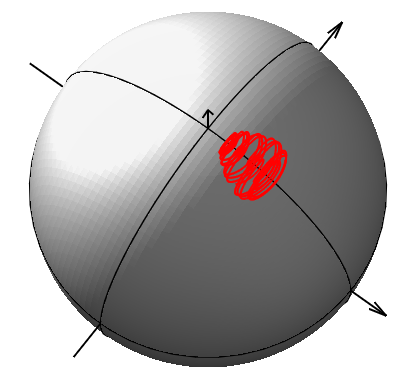
\includegraphics[width = \linewidth]{../pictures/HarmGroundState00/plot_J=26.png}
	    \caption{J=26}
	  \end{subfigure}
	\end{figure}
  \end{block}
\end{frame}

\begin{frame}{\small Траектории конца вектора углового момента в полномерной модели с потенциалом Морзе в основном состоянии}
  \begin{block}{}
  	\begin{figure}
	  \begin{subfigure}{0.25\textwidth}
	    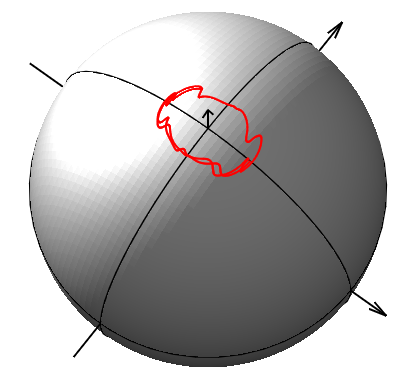
\includegraphics[width = \linewidth]{../pictures/MorseGroundState00/plot_J=15.png}
	    \caption{J=15}
	  \end{subfigure}
	  \begin{subfigure}{0.25\textwidth}
	    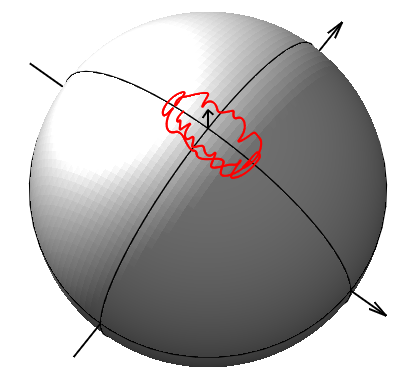
\includegraphics[width = \linewidth]{../pictures/MorseGroundState00/plot_J=20.png}
	    \caption{J=20}
	  \end{subfigure}
	  \begin{subfigure}{0.25\textwidth}
	    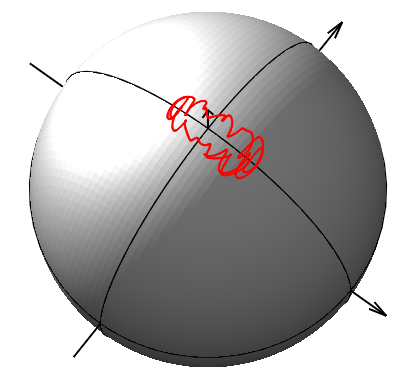
\includegraphics[width = \linewidth]{../pictures/MorseGroundState00/plot_J=25.png}
	    \caption{J=25}
	  \end{subfigure}
	  \begin{subfigure}{0.25\textwidth}
	    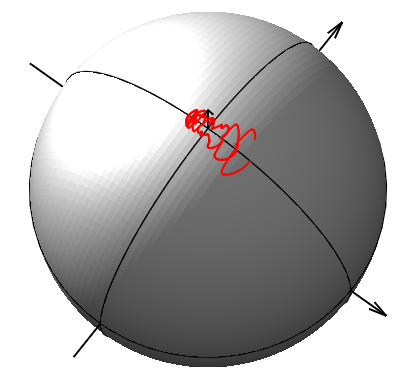
\includegraphics[width = \linewidth]{../pictures/MorseGroundState00/plot_J=28.png}
	    \caption{J=28}
	  \end{subfigure}
	  \begin{subfigure}{0.25\textwidth}
	    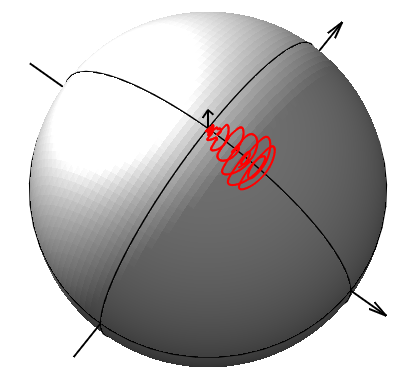
\includegraphics[width = \linewidth]{../pictures/MorseGroundState00/plot_J=29.png}
	    \caption{J=29}
	  \end{subfigure}
	  \begin{subfigure}{0.25\textwidth}
	    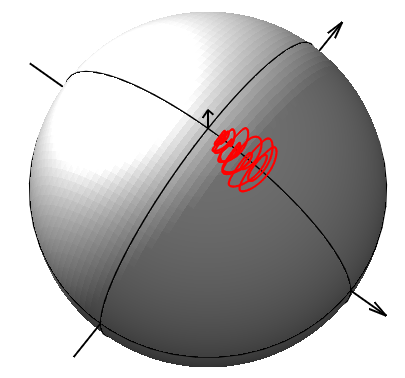
\includegraphics[width = \linewidth]{../pictures/MorseGroundState00/plot_J=30.png}
	    \caption{J=30}
	  \end{subfigure}
	 \end{figure}
  \end{block}
\end{frame}

\begin{frame}{Колебательно-вращательное движение из лабораторной системы отсчета}
\begin{center}
\begin{tikzpicture}
\node (ham1) [hamilton] {$\mathbf{J}, \mathbf{p}, r_1, r_2, q$};
\node (lag1) [lagrange, below = 0.5 cm of ham1] {$\mathbf{\Omega}, \mathbf{\dot{q}}$};
\node (eq1) [equations, minimum width = 2cm, text width = 2cm, below right = 0.1 cm and 0.5 cm of ham1] {$\bba, \bbA, \bbI$};

\node (eq2) [equations, minimum width = 4cm, text width = 4cm, below = 0.5 cm of lag1] {$
\left\{
\begin{aligned}
\mathbf{\dot{R}}_1 + \left[ \mathbf{\Omega} \times \mathbf{R}_1 \right] = \mathbf{\dot{r}}_1 \\
\mathbf{\dot{R}}_2 + \left[ \mathbf{\Omega} \times \mathbf{R}_2 \right] = \mathbf{\dot{r}}_2
\end{aligned}
\right.
$};

\node (res) [result, minimum width = 2 cm, text width = 2cm, right = 0.5 cm of eq2] {$\mathbf{R}_1, \mathbf{R}_2$};

\draw [arrow] (ham1) -- (lag1);
\draw [arrow] (ham1) -| (eq1);
\draw [arrow] (eq1) |- (lag1);
\draw [arrow] (lag1) -- (eq2);
\draw [arrow] (eq2) -- (res);

\begin{scope}[on background layer]
  \node [fill = BurntOrange!20, fit = (ham1) (lag1) (eq1) (eq2) (res)] {};
\end{scope}
\end{tikzpicture}
\end{center}
\end{frame}

\begin{frame}{Выводы}
\begin{itemize}
\item Описан метод получения точного колебательно-вращательного гамильтониана. \\
\item Получены гамильтонианы для одномерной и полномерной моделей трехатомной гидрида. \\ 
\item Получены поверхности вращательной энергии для одномерной модели. \\
\item Описано явление бифуркации с точки зрения перестройки поверхности вращательной энергии. \\
\item Получены классические траектории в различных колебательных состояниях.
\end{itemize}
\end{frame}

\begin{frame}{}
\begin{center}
\Huge Спасибо за внимание!
\end{center}
\end{frame}

\end{document}